\documentclass{scrartcl}
\usepackage{graphicx,tikz}
\usepackage{siunitx}
\usepackage[graphics,tightpage,active]{preview}
\newlength\imagewidth
\newlength\imagescale
\begin{document}
%%%%%%%%%%%%%%%%%%%%%%%%%%
	\newcommand{\imsize}{\linewidth}
	\pgfmathsetlength{\imagewidth}{\imsize}
	\pgfmathsetlength{\imagescale}{\imagewidth/1379}
	\def\x{852} % scalebar-x at golden ratio of x=1379px
	\def\y{898} % scalebar-y at 90% of height of y=998px
\begin{preview}
	\begin{tikzpicture}[x=\imagescale,y=-\imagescale]
		\node[anchor=north west, inner sep=0pt, outer sep=0pt] at (0,0) {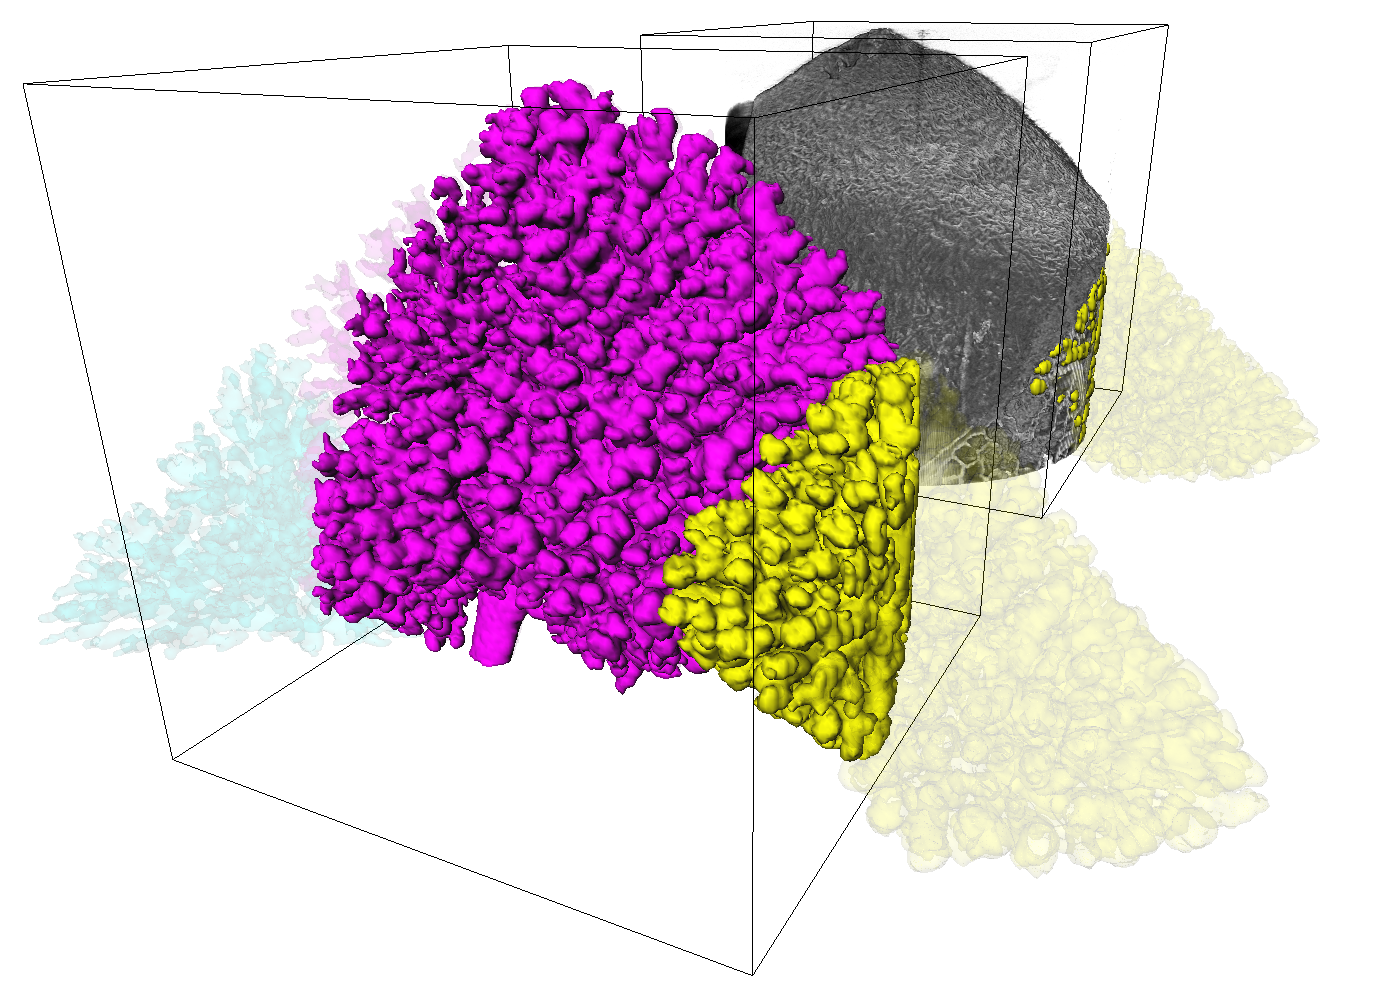
\includegraphics[width=\imagewidth]{../img/conv_vs_wfs/scan-conventional}};
		% 618px = 1.5155mm > 100px = 245um > 204px = 500um, 41px = 100um
		%\draw[color=red,|-|,thick] (174,761) -- (753,977) node [sloped,midway,above] {\SI{1.5155}{\milli\meter} (1024px)};
		\draw[|-|,thick] (\x,\y) -- (\x+204,\y) node [fill=white, semitransparent, midway, above] {\SI{500}{\micro\meter}};
		\draw[|-|,thick] (\x,\y) -- (\x+204,\y) node [midway, above]{\SI{500}{\micro\meter}};
	\draw[anchor=south west] (0,998) node [fill=white, semitransparent] {(a)} node {(a)};
	\end{tikzpicture}
	\begin{tikzpicture}[x=\imagescale,y=-\imagescale]
		\node[anchor=north west, inner sep=0pt, outer sep=0pt] at (0,0) 	{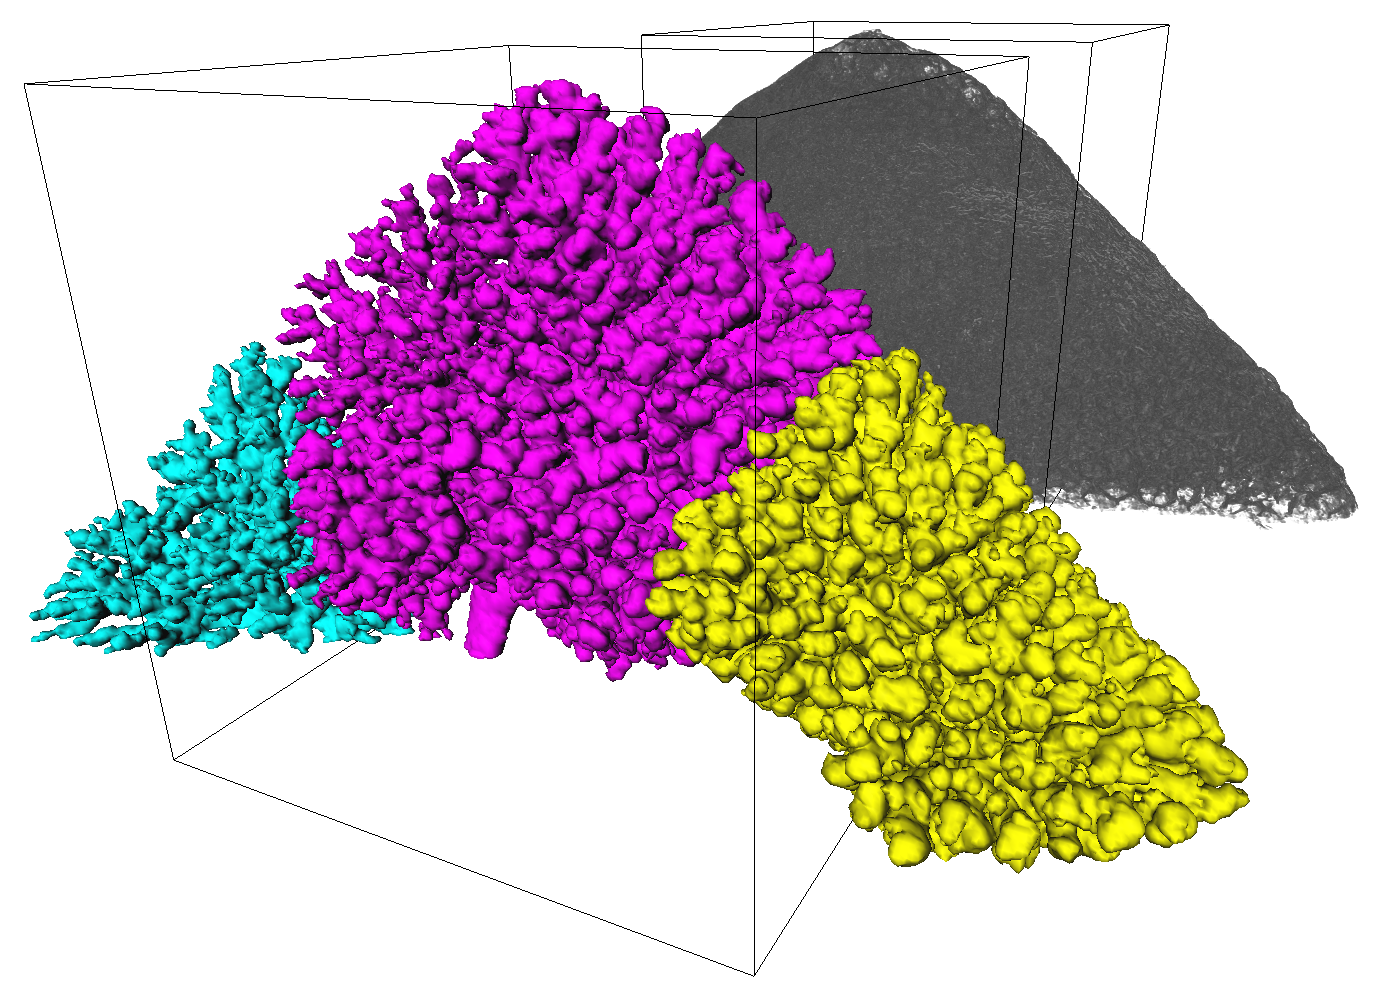
\includegraphics[width=\imagewidth]{../img/conv_vs_wfs/scan-widefield}};
		% 620px = 1.5155mm > 100px = 245um > 204px = 500um, 41px = 100um
		%\draw[color=red,|-|,thick] (174,761) -- (755,977) node [sloped,midway,above] {\SI{1.5155}{\milli\meter} (1024px)};
		\draw[|-|,thick] (\x,\y) -- (\x+204,\y) node [fill=white, semitransparent, midway, above] {\SI{500}{\micro\meter}};
		\draw[|-|,thick] (\x,\y) -- (\x+204,\y) node [midway, above]{\SI{500}{\micro\meter}};
		\draw[anchor=south west] (0,998) node [fill=white, semitransparent] {(b)} node {(b)};
	\end{tikzpicture}
\end{preview}
%%%%%%%%%%%%%%%%%%%%%%%%%%
\end{document}